\PassOptionsToPackage{unicode=true}{hyperref} % options for packages loaded elsewhere
\PassOptionsToPackage{hyphens}{url}
%
\documentclass[]{article}
\usepackage{lmodern}
\usepackage{amssymb,amsmath}
\usepackage{ifxetex,ifluatex}
\usepackage{fixltx2e} % provides \textsubscript
\ifnum 0\ifxetex 1\fi\ifluatex 1\fi=0 % if pdftex
  \usepackage[T1]{fontenc}
  \usepackage[utf8]{inputenc}
  \usepackage{textcomp} % provides euro and other symbols
\else % if luatex or xelatex
  \usepackage{unicode-math}
  \defaultfontfeatures{Ligatures=TeX,Scale=MatchLowercase}
\fi
% use upquote if available, for straight quotes in verbatim environments
\IfFileExists{upquote.sty}{\usepackage{upquote}}{}
% use microtype if available
\IfFileExists{microtype.sty}{%
\usepackage[]{microtype}
\UseMicrotypeSet[protrusion]{basicmath} % disable protrusion for tt fonts
}{}
\IfFileExists{parskip.sty}{%
\usepackage{parskip}
}{% else
\setlength{\parindent}{0pt}
\setlength{\parskip}{6pt plus 2pt minus 1pt}
}
\usepackage{hyperref}
\hypersetup{
            pdftitle={Energy-aware Timing Analysis of Intermittent Execution},
            pdfauthor={Ferhat Erata; Sinan Yıldırım; Arda Göknil; Ruzica Piskac; Jakub Szefer},
            pdfborder={0 0 0},
            breaklinks=true}
\urlstyle{same}  % don't use monospace font for urls
\usepackage[margin=1in]{geometry}
\usepackage{color}
\usepackage{fancyvrb}
\newcommand{\VerbBar}{|}
\newcommand{\VERB}{\Verb[commandchars=\\\{\}]}
\DefineVerbatimEnvironment{Highlighting}{Verbatim}{commandchars=\\\{\}}
% Add ',fontsize=\small' for more characters per line
\usepackage{framed}
\definecolor{shadecolor}{RGB}{248,248,248}
\newenvironment{Shaded}{\begin{snugshade}}{\end{snugshade}}
\newcommand{\AlertTok}[1]{\textcolor[rgb]{0.94,0.16,0.16}{#1}}
\newcommand{\AnnotationTok}[1]{\textcolor[rgb]{0.56,0.35,0.01}{\textbf{\textit{#1}}}}
\newcommand{\AttributeTok}[1]{\textcolor[rgb]{0.77,0.63,0.00}{#1}}
\newcommand{\BaseNTok}[1]{\textcolor[rgb]{0.00,0.00,0.81}{#1}}
\newcommand{\BuiltInTok}[1]{#1}
\newcommand{\CharTok}[1]{\textcolor[rgb]{0.31,0.60,0.02}{#1}}
\newcommand{\CommentTok}[1]{\textcolor[rgb]{0.56,0.35,0.01}{\textit{#1}}}
\newcommand{\CommentVarTok}[1]{\textcolor[rgb]{0.56,0.35,0.01}{\textbf{\textit{#1}}}}
\newcommand{\ConstantTok}[1]{\textcolor[rgb]{0.00,0.00,0.00}{#1}}
\newcommand{\ControlFlowTok}[1]{\textcolor[rgb]{0.13,0.29,0.53}{\textbf{#1}}}
\newcommand{\DataTypeTok}[1]{\textcolor[rgb]{0.13,0.29,0.53}{#1}}
\newcommand{\DecValTok}[1]{\textcolor[rgb]{0.00,0.00,0.81}{#1}}
\newcommand{\DocumentationTok}[1]{\textcolor[rgb]{0.56,0.35,0.01}{\textbf{\textit{#1}}}}
\newcommand{\ErrorTok}[1]{\textcolor[rgb]{0.64,0.00,0.00}{\textbf{#1}}}
\newcommand{\ExtensionTok}[1]{#1}
\newcommand{\FloatTok}[1]{\textcolor[rgb]{0.00,0.00,0.81}{#1}}
\newcommand{\FunctionTok}[1]{\textcolor[rgb]{0.00,0.00,0.00}{#1}}
\newcommand{\ImportTok}[1]{#1}
\newcommand{\InformationTok}[1]{\textcolor[rgb]{0.56,0.35,0.01}{\textbf{\textit{#1}}}}
\newcommand{\KeywordTok}[1]{\textcolor[rgb]{0.13,0.29,0.53}{\textbf{#1}}}
\newcommand{\NormalTok}[1]{#1}
\newcommand{\OperatorTok}[1]{\textcolor[rgb]{0.81,0.36,0.00}{\textbf{#1}}}
\newcommand{\OtherTok}[1]{\textcolor[rgb]{0.56,0.35,0.01}{#1}}
\newcommand{\PreprocessorTok}[1]{\textcolor[rgb]{0.56,0.35,0.01}{\textit{#1}}}
\newcommand{\RegionMarkerTok}[1]{#1}
\newcommand{\SpecialCharTok}[1]{\textcolor[rgb]{0.00,0.00,0.00}{#1}}
\newcommand{\SpecialStringTok}[1]{\textcolor[rgb]{0.31,0.60,0.02}{#1}}
\newcommand{\StringTok}[1]{\textcolor[rgb]{0.31,0.60,0.02}{#1}}
\newcommand{\VariableTok}[1]{\textcolor[rgb]{0.00,0.00,0.00}{#1}}
\newcommand{\VerbatimStringTok}[1]{\textcolor[rgb]{0.31,0.60,0.02}{#1}}
\newcommand{\WarningTok}[1]{\textcolor[rgb]{0.56,0.35,0.01}{\textbf{\textit{#1}}}}
\usepackage{longtable,booktabs}
% Fix footnotes in tables (requires footnote package)
\IfFileExists{footnote.sty}{\usepackage{footnote}\makesavenoteenv{longtable}}{}
\usepackage{graphicx,grffile}
\makeatletter
\def\maxwidth{\ifdim\Gin@nat@width>\linewidth\linewidth\else\Gin@nat@width\fi}
\def\maxheight{\ifdim\Gin@nat@height>\textheight\textheight\else\Gin@nat@height\fi}
\makeatother
% Scale images if necessary, so that they will not overflow the page
% margins by default, and it is still possible to overwrite the defaults
% using explicit options in \includegraphics[width, height, ...]{}
\setkeys{Gin}{width=\maxwidth,height=\maxheight,keepaspectratio}
\setlength{\emergencystretch}{3em}  % prevent overfull lines
\providecommand{\tightlist}{%
  \setlength{\itemsep}{0pt}\setlength{\parskip}{0pt}}
\setcounter{secnumdepth}{5}
% Redefines (sub)paragraphs to behave more like sections
\ifx\paragraph\undefined\else
\let\oldparagraph\paragraph
\renewcommand{\paragraph}[1]{\oldparagraph{#1}\mbox{}}
\fi
\ifx\subparagraph\undefined\else
\let\oldsubparagraph\subparagraph
\renewcommand{\subparagraph}[1]{\oldsubparagraph{#1}\mbox{}}
\fi

% set default figure placement to htbp
\makeatletter
\def\fps@figure{htbp}
\makeatother

\renewcommand{\contentsname}{}\vspace{-.5cm}
\usepackage{etoolbox}
\makeatletter
\providecommand{\subtitle}[1]{% add subtitle to \maketitle
  \apptocmd{\@title}{\par {\large #1 \par}}{}{}
}
\makeatother
\usepackage[]{natbib}
\bibliographystyle{plainnat}

\title{\vspace{-1.5cm}Energy-aware Timing Analysis of Intermittent Execution}
\providecommand{\subtitle}[1]{}
\subtitle{Experimentation and Evaluation Plan}
\author{Ferhat Erata \and Sinan Yıldırım \and Arda Göknil \and Ruzica Piskac \and Jakub Szefer}
\date{28 February 2021\vspace{-1.5cm}}

\begin{document}
\maketitle

{
\setcounter{tocdepth}{3}
\tableofcontents
}
\hypertarget{testbed-applications}{%
\section{Testbed Applications}\label{testbed-applications}}

To demonstrate the usefulness of the approach, we aim at developing one or two sensing applications. The first candidate is anomaly detection through audio sensing.

The other candidate that we discussed is motion detection similar to anamoly detection. In these two scenarios, we don't plan to connect a real sensor or a transmitter to the launchpad. Instead, we will simulate the energy consumption and timing by delays and timers as well as the data received or transmitted through embedding sample or generating random data.

Apart from sensing application, we can elaborate the evaluation on security applications using computational intensive tasks such as data encryption, decryption and hashing algorithms if we have enough time or we can analyze security in the context of intermittent execution in a follow-up work.

We composed a set of \texttt{Tasks} that are frequently used in resource constrained embedded system development. They are open-source implementation of the following algorithms: \emph{FFT}, \emph{JPEG}, \emph{SHA}, \emph{RSA}, \emph{AES}, \emph{CRC}, \emph{QSort}, and \emph{bitcount}. We managed to successfully deploy and run those algorithms on the MSP430FR5994 launchpad.

\begin{longtable}[]{@{}llcccl@{}}
\toprule
Task & Explanation & Checkpointed & Measured & Analyzed & Exp. Timing\tabularnewline
\midrule
\endhead
FFT & Fast Fourier Transform & \(\checkmark\) & & & 3/s\tabularnewline
JPEG & Jpeg image compression & & & &\tabularnewline
SHA & Secure Hash Algorithm & \(\checkmark\) & & & 10/s\tabularnewline
CRC & Cyclic Redundancy Check & \(\checkmark\) & & &\tabularnewline
AES & Advanced Encryption Standard & \(\checkmark\) & & &\tabularnewline
RSA & RSA public-key cryptosystem & & & &\tabularnewline
QSort & Quicksort Algorithm & & & &\tabularnewline
BitCount & Bit Count Algorithms & & & &\tabularnewline
\bottomrule
\end{longtable}

The \texttt{compute()} part of the embedded application is the stage of the application where we assume the embedded programmer places checkpoints. The \texttt{ETAP} will be able to infer the probability distribution of the timing of \texttt{compute()} stage, from sensing to transmit; it may also report the rate of successful runs of the application (such as the 68\%, 95\% and 99.7\% success rates); or it may check whether a timing constraint is satisfied or not within a confidence interval.

\begin{longtable}[]{@{}llccc@{}}
\toprule
Testbed Application & Tasks & Checkpointed & Measured & Analyzed\tabularnewline
\midrule
\endhead
Audio Sensing \& Anomaly Detection {[}\ref{app-1}{]} & FFT, & & &\tabularnewline
Encrypted Communication {[}\ref{app-2}{]} & SHA, AES & & &\tabularnewline
\bottomrule
\end{longtable}

\hypertarget{sensing-applications}{%
\subsection{Sensing Applications}\label{sensing-applications}}

\texttt{Sense()\ -\textgreater{}\ Compute()\ -\textgreater{}\ Transmit()}

\begin{itemize}
\tightlist
\item
  \emph{FFT}: Fast-Fourier Transform.
\item
  \emph{JPEG}: Graphic Image Compression.
\end{itemize}

\hypertarget{app-1}{%
\subsubsection*{Application 1: Audio Sensing and Anomaly Detection}\label{app-1}}
\addcontentsline{toc}{subsubsection}{Application 1: Audio Sensing and Anomaly Detection}

\begin{enumerate}
\def\labelenumi{\arabic{enumi}.}
\tightlist
\item
  Sample Audio (Embedded test data or random-generated data).
\item
  Perform \emph{FFT} (Time to Frequency)
\item
  Detect an event (anomaly): The frequency of the sample exceeds the threshold.
\item
  Send (raise a pin) it in 10 seconds or \texttt{Green\ (normal)\ Red\ (anomaly)}
\item
  Go to 1st step.
\end{enumerate}

\hypertarget{application-2-motion-detection}{%
\subsubsection*{Application 2: Motion Detection}\label{application-2-motion-detection}}
\addcontentsline{toc}{subsubsection}{Application 2: Motion Detection}

\begin{enumerate}
\def\labelenumi{\arabic{enumi}.}
\tightlist
\item
  Capture 1st Frame (RGB data format) 640x480 RGB array -\textgreater{} JPEG array
\item
  Hash frame 1 \emph{SHA} (or \emph{jpeg} encoder -compression-)
\item
  Capture 2nd Frame (RGB data format)
\item
  Hash frame 2 \emph{SHA} (or \emph{jpeg} encoder -compression-)
\item
  Compare hashes (or compare jpegs)
\item
  Transmit (if the anomaly detected, blink the LED twice)
\item
  Go to 1st step.
\end{enumerate}

\hypertarget{security-applications}{%
\subsection{Security Applications}\label{security-applications}}

\texttt{Receive()\ -\textgreater{}\ Compute()\ -\textgreater{}\ Transmit()}

\begin{itemize}
\tightlist
\item
  \emph{RSA} asymmetric encryption (public/private key)
\item
  \emph{AES} symmetric encryption (shared key)
\item
  \emph{SHA} authentication, hashing
\item
  \emph{CRC} Cyclic Redundancy Check (CRC)
\end{itemize}

\hypertarget{application-1-authentication-access-control}{%
\subsubsection*{Application 1: Authentication (Access control)}\label{application-1-authentication-access-control}}
\addcontentsline{toc}{subsubsection}{Application 1: Authentication (Access control)}

\begin{enumerate}
\def\labelenumi{\arabic{enumi}.}
\tightlist
\item
  Wait for receiving a signal (when pushed a button send a random secret message from an array)
\item
  \emph{SHA} (check the signature, if it is authentic, blink the LED)
\item
  Signal
\end{enumerate}

\hypertarget{app-2}{%
\subsubsection*{Application 2: Encrypted Communication}\label{app-2}}
\addcontentsline{toc}{subsubsection}{Application 2: Encrypted Communication}

\begin{enumerate}
\def\labelenumi{\arabic{enumi}.}
\tightlist
\item
  Wait for receiving a signal
\item
  Analyze()
\item
  \emph{AES} (Encrypt)
\item
  Transmit
\item
  Go to 1st step.
\end{enumerate}

\hypertarget{application-3-error-correcting-of-signed-messages}{%
\subsubsection*{Application 3: Error Correcting of signed messages}\label{application-3-error-correcting-of-signed-messages}}
\addcontentsline{toc}{subsubsection}{Application 3: Error Correcting of signed messages}

\begin{enumerate}
\def\labelenumi{\arabic{enumi}.}
\tightlist
\item
  Wait for receiving a message
\item
  \emph{CRC} (checksum)
\item
  analyze the message
\item
  sign the signal
\item
  send the signal (blink LED)
\item
  Go to 1st step.
\end{enumerate}

\hypertarget{hardware-setup}{%
\section{Hardware Setup}\label{hardware-setup}}

\hypertarget{checkpointing-inside-tasks}{%
\subsection{Checkpointing inside Tasks}\label{checkpointing-inside-tasks}}

Batteryless devices, instead of getting energy from the power grid or a battery, harvest their energy from their environment (e.g., sunlight or radio waves). Energy harvesting devices replace batteries with a small energy storage capacitor. We can consider the size of the capacitor as being proportional to the duration of computation.

We run the \emph{SHA} task successfully using the checkpointing library that Sinan's PhD Student Eren Yildiz developed. We specified a \texttt{fixed\ number\ of\ cycles} and set a timer duration to fire soft reset to simulate \texttt{power\ failures}. After soft reset, we also set a \texttt{random\ delays} simulating the recharge period of the capacitor. After a power failure, with the minimum overhead, the runtime restores the execution from the last checkpointed region. During the computation we turn on the \emph{LED1} (Red) and during the power failure we turn the LED1 off.

In the application development, one of the challenges is to place checkpoints (such as in \emph{FFT} and \emph{JPEG} tasks) carefully so that we should maintain forward progress. The total number of cycles executed between two consecutive checkpointed region should always consume less energy than the maximum stored energy.

So I might cite some things \citep{Shea2014}

\hypertarget{considerations-for-clock-speed}{%
\subsection{Considerations for Clock Speed}\label{considerations-for-clock-speed}}

1 MHz or 8 MHz

Assuming your CPU frequency is 1Mz , each cycle takes 1uS. so for 1 second you have to use the count 1000000.

There is a direct tradeoff between clock speed and energy consumption. What should we set for the clock speed? 8MHz?

\hypertarget{device-setup}{%
\subsection{Device Setup}\label{device-setup}}

\begin{itemize}
\item
  In our evaluation, we use TI's msp430FR6989 development board, the latest released version of TI boards that includes an embedded byte addressable persistent memory. The microcontroller is a 16-Bit RISC architecture and is clocked at 8-MHz. It has 2KB of SRAM or volatile memory, and an effective 82KB of Ferroelectric RAM (FRAM) -- a non-volatile, byte-addressable memory. The 82KB of FRAM is shared between the application code and application data allocated as persistent. The memory model is flat, meaning a single contiguous address space is used and the CPU directly addresses SRAM, FRAM, etc. The CPU supports a 20-bit addressing mode (msp430x) required for accessing the full address space, which we activate by default for our experiments.
\item
  We applied CleanCut to real code on real energy-harvesting hardware. We used the WISP energy- harvesting device, which has an 8MHz MSP430FR5969 MCU with 64KB of non-volatile memory and a 47\(\mu\)F capacitor. We powered the WISP wirelessly using a ThingMagic Astra-EX RFID reader at 16 dBm. We fixed the WISP 45 cm from the power antenna, parallel to its surface.
\item
  The WISPCam's MSP430FR5969 microcontroller has a 64KB on-chip FRAM memory that supports 48 Mb/s data transfer from the camera to the microcontroller while burning only a few milliwatts of power. WISPCam main board, based heavily on the WISP 5.0. An AVX BestCap series supercapacitor allows the WISPCam to accumulate the 20 mJ necessary for image capture and transfer. we found that at least 10 mJ of energy is required to capture and store a 176*144 pixel (QCIF) gray scale image such as those seen in Figure 12 (Images with higher contrast or higher resolution will require expending more energy). We select a 6.08 mF supercapacitor and target 20 mJs of usable energy.
\item
  We implement Ratchet using the LLVM compiler infrastructure. Beyond verifying that Ratchet output executes correctly on an ARM development board, we build an ARMv6-M energy-harvesting simulator, with wholly non-volatile memory. We use an average lifetime of 100 ms to match the setup of previous works. With an average lifetime of 100 ms running with a 24 MHz clock, this gives us a mean lifetime of 2,400,000 cycles. Before each bout of execution, the simulator samples from a Gaussian whose mean is the desired mean lifetime (in cycles) and uses that value as the number of clock cycles to execute for before inducing the next power cycle. To simulate a power cycle, we clear the register values.
\end{itemize}

\hypertarget{energy-harvesting-simulator-on-msp430}{%
\subsection{Energy Harvesting Simulator on MSP430}\label{energy-harvesting-simulator-on-msp430}}

An energy-harvesting simulator is required because of the difficulties associated with developing and debugging intermittently powered devices. Using a cycle accurate simulator we are able to simulate failures with a probability distribution that can model the true frequency and effects of power failures experienced by devices in the real world. Using a simulator also allows us to take precise measurements of how much progress a program makes per power cycle, and the cycles consumed by re-execution.

\hypertarget{statistical-inference-of-the-instruction-based-energy-models}{%
\section{Statistical Inference of the Instruction-based Energy Models}\label{statistical-inference-of-the-instruction-based-energy-models}}

We should infer the probability density function of the energy consumption of each instruction types. Instructions work in MSP430 ISA with different operating modes. Therefore, the energy trace collection should also consider addressing modes of the instructions.

\hypertarget{energy-traces-collected-from-the-energytrace-of-code-composer-studio.}{%
\subsection{Energy Traces collected from the EnergyTrace++ of Code Composer Studio.}\label{energy-traces-collected-from-the-energytrace-of-code-composer-studio.}}

We aim to profile about 20 different instruction, each of them should run at least 100 times. The problem is there is no commandline interface of API for us to write a script. Each test requires us to click a set of buttons on the Eclipse IDE (CCS Studio). We are working on a python script that automated mouse click events.

Here is an example trace data. We can also measure specific execution intervals through the graphical user interface of the Code Composer Studio.

What is the causal relationship here? What is the explanatory (x:independent), response(y:dependent variable)

\begin{Shaded}
\begin{Highlighting}[]
\NormalTok{Time (ns),Current (nA),Voltage (mV),Energy (uJ),DSR}
\StringTok{"0"}\NormalTok{      ,}\StringTok{"3356900"}\NormalTok{   ,}\StringTok{"3287"}\NormalTok{      ,}\StringTok{"50.1"}\NormalTok{     ,}\StringTok{"0x3E1017E80000830"}
\StringTok{"902000"}\NormalTok{ ,}\StringTok{"3356900"}\NormalTok{   ,}\StringTok{"3272"}\NormalTok{      ,}\StringTok{"60.5"}\NormalTok{     ,}\StringTok{""}
\StringTok{"1744000"}\NormalTok{,}\StringTok{"3356900"}\NormalTok{   ,}\StringTok{"3277"}\NormalTok{      ,}\StringTok{"70.1"}\NormalTok{     ,}\StringTok{""}
\StringTok{"2588000"}\NormalTok{,}\StringTok{"3356900"}\NormalTok{   ,}\StringTok{"3272"}\NormalTok{      ,}\StringTok{"79.2"}\NormalTok{     ,}\StringTok{""}
\StringTok{"3431000"}\NormalTok{,}\StringTok{"3356900"}\NormalTok{   ,}\StringTok{"3276"}\NormalTok{      ,}\StringTok{"88.8"}\NormalTok{     ,}\StringTok{""}
\StringTok{"4530000"}\NormalTok{,}\StringTok{"3410900"}\NormalTok{   ,}\StringTok{"3273"}\NormalTok{      ,}\StringTok{"101.1"}\NormalTok{    ,}\StringTok{""}
\NormalTok{...}
\end{Highlighting}
\end{Shaded}

\hypertarget{sampling-add-instruction}{%
\subsection{Sampling ADD instruction}\label{sampling-add-instruction}}

Sample the instructions wrt. addressing modes.

\begin{enumerate}
\def\labelenumi{\arabic{enumi}.}
\tightlist
\item
  Measure the energy consumption \(E_{total}\)
\end{enumerate}

\begin{Shaded}
\begin{Highlighting}[]
\CommentTok{// start the energy profiling here}
\ControlFlowTok{while}\NormalTok{(}\DecValTok{1000}\NormalTok{)\{}
\NormalTok{    ...}
\NormalTok{  __asm__ __volatile__ (}\StringTok{" ADD R3,0(R15)"}\NormalTok{);}
\NormalTok{\}}
\CommentTok{// stop the energy profiling on halt}
\end{Highlighting}
\end{Shaded}

\begin{enumerate}
\def\labelenumi{\arabic{enumi}.}
\setcounter{enumi}{1}
\tightlist
\item
  Measure the energy consumption \(E_{overhead}\)
\end{enumerate}

\begin{Shaded}
\begin{Highlighting}[]
\CommentTok{// start the energy profiling here}
\ControlFlowTok{while}\NormalTok{(}\DecValTok{1000}\NormalTok{)\{}
\NormalTok{ ; }\CommentTok{// noop instruction}
\NormalTok{\}}
\CommentTok{// stop the energy profiling on halt}
\end{Highlighting}
\end{Shaded}

\(E_{ADD} = (E_{total} - E_{while} - E_{startup}) / 1000\)

\begin{enumerate}
\def\labelenumi{\arabic{enumi}.}
\setcounter{enumi}{2}
\tightlist
\item
  Repeat sampling x100.
\end{enumerate}

uj (one decimal precision)

\begin{enumerate}
\def\labelenumi{\arabic{enumi}.}
\tightlist
\item
  create a vector from samples
\end{enumerate}

\begin{Shaded}
\begin{Highlighting}[]
\NormalTok{add <-}\StringTok{ }\KeywordTok{c}\NormalTok{(}\FloatTok{11.3}\NormalTok{, }\FloatTok{12.5}\NormalTok{, ...) }\CommentTok{# list of 100 samples}
\end{Highlighting}
\end{Shaded}

\begin{enumerate}
\def\labelenumi{\arabic{enumi}.}
\setcounter{enumi}{1}
\tightlist
\item
  fit a normal distribution
\end{enumerate}

\begin{Shaded}
\begin{Highlighting}[]
\CommentTok{## reproducible example}
\KeywordTok{set.seed}\NormalTok{(}\DecValTok{0}\NormalTok{); x <-}\StringTok{ }\KeywordTok{rnorm}\NormalTok{(}\DecValTok{100}\NormalTok{)}
\CommentTok{## using MASS}

\KeywordTok{library}\NormalTok{(MASS)}
\NormalTok{fit <-}\StringTok{ }\KeywordTok{fitdistr}\NormalTok{(x, }\StringTok{"normal"}\NormalTok{)}
\KeywordTok{class}\NormalTok{(fit)}
\end{Highlighting}
\end{Shaded}

\begin{verbatim}
## [1] "fitdistr"
\end{verbatim}

\begin{Shaded}
\begin{Highlighting}[]
\CommentTok{# [1] "fitdistr"}

\NormalTok{para <-}\StringTok{ }\NormalTok{fit}\OperatorTok{$}\NormalTok{estimate}
\CommentTok{#         mean            sd}
\CommentTok{#-0.0002000485  0.9886248515}

\KeywordTok{hist}\NormalTok{(x, }\DataTypeTok{prob =} \OtherTok{TRUE}\NormalTok{, }\DataTypeTok{breaks =} \DecValTok{20}\NormalTok{, }\DataTypeTok{ylab =} \StringTok{""}\NormalTok{, }\DataTypeTok{xlab =} \StringTok{""}\NormalTok{, }\DataTypeTok{main =} \StringTok{""}\NormalTok{)}
\KeywordTok{curve}\NormalTok{(}\KeywordTok{dnorm}\NormalTok{(x, para[}\DecValTok{1}\NormalTok{], para[}\DecValTok{2}\NormalTok{]), }\DataTypeTok{col =} \DecValTok{2}\NormalTok{, }\DataTypeTok{add =} \OtherTok{TRUE}\NormalTok{)}
\end{Highlighting}
\end{Shaded}

\begin{figure}
\centering
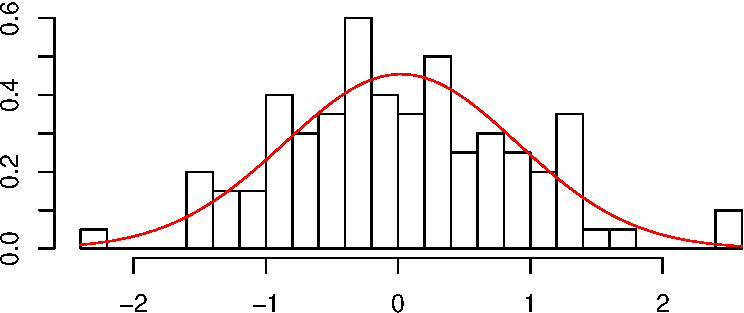
\includegraphics{/home/ferhat/git/analysis-framework-standalone-application/experiments/report/report_files/figure-latex/unnamed-chunk-1-1.pdf}
\caption{\label{fig:unnamed-chunk-1}The instruction-based energy model for Add instruction.}
\end{figure}

\hypertarget{sampling-mov-instruction}{%
\subsection{Sampling MOV instruction}\label{sampling-mov-instruction}}

there are several modes to consider:

\begin{itemize}
\tightlist
\item
  store to volatile ram (SRAM)
\item
  store to nv ram (FRAM)
\item
  store to register
\end{itemize}

maybe this will lead to a bimodal distribution

\hypertarget{other-methods-to-derive-instruction-based-energy-models}{%
\section{Other methods to derive instruction-based energy models}\label{other-methods-to-derive-instruction-based-energy-models}}

\hypertarget{optimization-model}{%
\subsection{Optimization Model}\label{optimization-model}}

Although the previous approach may successfully infer probabilistic models for each instruction types, they are still MPS430 ISA. However, the probabilistic symbolic execution engine only runs on LLVM IR. There is no one-to-one correspondence with the architecture independent representation of the instruction set, and the MSP420 instruction set. Nevertheless, we can construct an optimization problem as the following: first we can collect samples from a set of benchmarks applications; for each program, we can sample 100 and take its expectation; and we can count the frequency of each instruction type; and finally construct linear equations

Here is an R program solving linear equations

\begin{Shaded}
\begin{Highlighting}[]
\CommentTok{#https://cran.r-project.org/web/packages/matlib/vignettes/linear-equations.html}
\KeywordTok{rm}\NormalTok{(}\DataTypeTok{list =} \KeywordTok{ls}\NormalTok{(}\DataTypeTok{all.names =} \OtherTok{TRUE}\NormalTok{)) }\CommentTok{#will clear all objects includes hidden objects.}
\KeywordTok{library}\NormalTok{(matlib)   }\CommentTok{# use the package}
\NormalTok{A <-}\StringTok{ }\KeywordTok{matrix}\NormalTok{(}\KeywordTok{c}\NormalTok{(}\DecValTok{1}\NormalTok{, }\DecValTok{1}\NormalTok{, }\DecValTok{1}\NormalTok{,}
              \DecValTok{1}\NormalTok{, }\DecValTok{2}\NormalTok{, }\DecValTok{1}\NormalTok{,}
              \DecValTok{2}\NormalTok{, }\DecValTok{1}\NormalTok{, }\DecValTok{1}\NormalTok{), }\DecValTok{3}\NormalTok{, }\DecValTok{3}\NormalTok{, }\DataTypeTok{byrow =} \OtherTok{TRUE}\NormalTok{)}
\KeywordTok{colnames}\NormalTok{(A) <-}\StringTok{ }\KeywordTok{c}\NormalTok{(}\StringTok{"alloca"}\NormalTok{, }\StringTok{"load"}\NormalTok{, }\StringTok{"store"}\NormalTok{) }\CommentTok{# "io.read", "io.write"}
\KeywordTok{rownames}\NormalTok{(A) <-}\StringTok{ }\KeywordTok{c}\NormalTok{(}\StringTok{"program.1"}\NormalTok{, }\StringTok{"program.2"}\NormalTok{, }\StringTok{"program.3"}\NormalTok{)}
\NormalTok{A}
\end{Highlighting}
\end{Shaded}

\begin{verbatim}
##           alloca load store
## program.1      1    1     1
## program.2      1    2     1
## program.3      2    1     1
\end{verbatim}

\begin{Shaded}
\begin{Highlighting}[]
\NormalTok{b <-}\StringTok{ }\KeywordTok{c}\NormalTok{(}\DecValTok{21}\NormalTok{, }\DecValTok{31}\NormalTok{, }\DecValTok{31}\NormalTok{) }\CommentTok{#1}
\KeywordTok{showEqn}\NormalTok{(A, b)}
\end{Highlighting}
\end{Shaded}

\begin{verbatim}
## 1*x1 + 1*x2 + 1*x3  =  21 
## 1*x1 + 2*x2 + 1*x3  =  31 
## 2*x1 + 1*x2 + 1*x3  =  31
\end{verbatim}

\begin{Shaded}
\begin{Highlighting}[]
\KeywordTok{Solve}\NormalTok{(A, b, }\DataTypeTok{fractions =} \OtherTok{TRUE}\NormalTok{)}
\end{Highlighting}
\end{Shaded}

\begin{verbatim}
## x1      =  10 
##   x2    =  10 
##     x3  =   1
\end{verbatim}

\begin{Shaded}
\begin{Highlighting}[]
\NormalTok{b <-}\StringTok{ }\KeywordTok{c}\NormalTok{(}\DecValTok{21}\NormalTok{, }\DecValTok{31}\NormalTok{, }\DecValTok{32}\NormalTok{) }\CommentTok{#2}
\KeywordTok{showEqn}\NormalTok{(A, b)}
\end{Highlighting}
\end{Shaded}

\begin{verbatim}
## 1*x1 + 1*x2 + 1*x3  =  21 
## 1*x1 + 2*x2 + 1*x3  =  31 
## 2*x1 + 1*x2 + 1*x3  =  32
\end{verbatim}

\begin{Shaded}
\begin{Highlighting}[]
\KeywordTok{Solve}\NormalTok{(A, b, }\DataTypeTok{fractions =} \OtherTok{TRUE}\NormalTok{)}
\end{Highlighting}
\end{Shaded}

\begin{verbatim}
## x1      =  11 
##   x2    =  10 
##     x3  =   0
\end{verbatim}

\begin{Shaded}
\begin{Highlighting}[]
\NormalTok{b <-}\StringTok{ }\KeywordTok{c}\NormalTok{(}\DecValTok{21}\NormalTok{, }\DecValTok{31}\NormalTok{, }\DecValTok{33}\NormalTok{) }\CommentTok{#3}
\KeywordTok{showEqn}\NormalTok{(A, b)}
\end{Highlighting}
\end{Shaded}

\begin{verbatim}
## 1*x1 + 1*x2 + 1*x3  =  21 
## 1*x1 + 2*x2 + 1*x3  =  31 
## 2*x1 + 1*x2 + 1*x3  =  33
\end{verbatim}

\begin{Shaded}
\begin{Highlighting}[]
\KeywordTok{Solve}\NormalTok{(A, b, }\DataTypeTok{fractions =} \OtherTok{TRUE}\NormalTok{)}
\end{Highlighting}
\end{Shaded}

\begin{verbatim}
## x1      =  12 
##   x2    =  10 
##     x3  =  -1
\end{verbatim}

Here the same procedure is modeled as a linear programming problem. The configuration is different.

\begin{Shaded}
\begin{Highlighting}[]
\CommentTok{# Linera Programming}
\CommentTok{# https://rstudio-pubs-static.s3.amazonaws.com/534936_8eeb46b4b20d47509e4dede705dbb1c4.html}
\KeywordTok{library}\NormalTok{(lpSolveAPI)}

\NormalTok{lps.model <-}\StringTok{ }\KeywordTok{make.lp}\NormalTok{(}\DecValTok{0}\NormalTok{, }\DecValTok{3}\NormalTok{) }\CommentTok{# define 3 variables, the constraints are added below}
\KeywordTok{add.constraint}\NormalTok{(lps.model, }\KeywordTok{c}\NormalTok{(}\DecValTok{6}\NormalTok{, }\DecValTok{2}\NormalTok{, }\DecValTok{4}\NormalTok{), }\StringTok{"<="}\NormalTok{, }\DecValTok{150}\NormalTok{)}
\KeywordTok{add.constraint}\NormalTok{(lps.model, }\KeywordTok{c}\NormalTok{(}\DecValTok{1}\NormalTok{, }\DecValTok{1}\NormalTok{, }\DecValTok{6}\NormalTok{), }\StringTok{">="}\NormalTok{, }\DecValTok{0}\NormalTok{)}
\KeywordTok{add.constraint}\NormalTok{(lps.model, }\KeywordTok{c}\NormalTok{(}\DecValTok{4}\NormalTok{, }\DecValTok{5}\NormalTok{, }\DecValTok{4}\NormalTok{), }\StringTok{"="}\NormalTok{, }\DecValTok{40}\NormalTok{)}
\CommentTok{# set objective function (default: find minimum)}
\KeywordTok{set.objfn}\NormalTok{(lps.model, }\KeywordTok{c}\NormalTok{(}\OperatorTok{-}\DecValTok{3}\NormalTok{, }\DecValTok{-4}\NormalTok{, }\DecValTok{-3}\NormalTok{))}
\CommentTok{# write model to a file}
\KeywordTok{write.lp}\NormalTok{(lps.model, }\StringTok{'model.lp'}\NormalTok{, }\DataTypeTok{type =} \StringTok{'lp'}\NormalTok{)}

\CommentTok{# these commands defines the model}
\CommentTok{# /* Objective function */}
\CommentTok{#   min: -3 C1 -4 C2 -3 C3;}
\CommentTok{#}
\CommentTok{# /* Constraints */}
\CommentTok{# +6 C1 +2 C2 +4 C3 <= 150;}
\CommentTok{# +  C1 +  C2 +6 C3 >=   0;}
\CommentTok{# +4 C1 +5 C2 +4 C3  =  40;}
\CommentTok{#}
\CommentTok{# writing it in the text file named 'model.lp'}
\KeywordTok{solve}\NormalTok{(lps.model)}

\CommentTok{# Retrieve the var values from a solved linear program model}
\KeywordTok{get.variables}\NormalTok{(lps.model)  }\CommentTok{# check with the solution above!}
\end{Highlighting}
\end{Shaded}

\hypertarget{instruction-based-model-from-block-based-mapping.}{%
\subsection{Instruction-based Model from Block-based Mapping.}\label{instruction-based-model-from-block-based-mapping.}}

Cemal hoca's method

\hypertarget{does-this-gap-pose-another-research-question}{%
\subsection{Does this gap pose another research question?}\label{does-this-gap-pose-another-research-question}}

Recent advances in security testing of embedded and IoT software focus on research having built on top of tools that rely on LLVM compiler infrastructure. While this technology is powerful and allows researchers to experiment, relieving them from implementation issues. Yet, these solutions might be difficult to apply in embedded and IoT domains which adopt different (and mostly proprietary) compiler and OS technologies. Investigate binary analysis ?? what are the drawbacks of binary analysis?

\hypertarget{statistical-inference-for-the-incoming-harvested-energy-model}{%
\section{Statistical Inference for the Incoming (Harvested) Energy Model}\label{statistical-inference-for-the-incoming-harvested-energy-model}}

We need to infer a probability density function for the harvested energy. It will be our stochastic incoming energy model as an input of the probabilistic symbolic execution engine.

I haven't investigated yet how to measure the voltage pin???

\begin{itemize}
\tightlist
\item
  We need to prepare a meaningful setup: 1 - 3 - 5 meters collect profiles; maybe 45 degrees. However, if the application's context is gunshot detection, then we need to at least 50 meters???
\end{itemize}

\hypertarget{resource-planning}{%
\section{Resource Planning}\label{resource-planning}}

\begin{enumerate}
\def\labelenumi{\arabic{enumi}.}
\tightlist
\item
  sampling and statistical inference:
\end{enumerate}

\begin{itemize}
\tightlist
\item
  instruction-based energy model (\texttt{1.5\ week}) : \texttt{Enes,\ Gokçin}
\item
  incoming (harvested) energy model (\texttt{1.5\ week}) : \texttt{Ferhat}
\end{itemize}

\begin{enumerate}
\def\labelenumi{\arabic{enumi}.}
\setcounter{enumi}{1}
\tightlist
\item
  application development
\end{enumerate}

\begin{itemize}
\tightlist
\item
  audio anomaly detection (\texttt{1\ week}): \texttt{Enes,\ Gökçin}
\item
  motion detection (\texttt{1\ week}): \texttt{Enes,\ Gökçin}
\end{itemize}

\begin{enumerate}
\def\labelenumi{\arabic{enumi}.}
\setcounter{enumi}{2}
\tightlist
\item
  intermittent execution semantics
\end{enumerate}

\begin{itemize}
\tightlist
\item
  development of the missing parts of the intermittent execution semantics (\texttt{1\ week)}: \texttt{Ferhat}
\item
  evaluating the probabilistic symbolic execution with the algorithms used in the applications; if necessary, introduce ways to increase the scalability such as state merging (\texttt{1\ week}): \texttt{Ferhat}
\end{itemize}

\begin{enumerate}
\def\labelenumi{\arabic{enumi}.}
\setcounter{enumi}{3}
\tightlist
\item
  Evaluation
\end{enumerate}

\begin{itemize}
\tightlist
\item
  final evaluation with the models (\texttt{1\ week}) : \texttt{Enes,\ Gökçin}
\end{itemize}

\begin{enumerate}
\def\labelenumi{\arabic{enumi}.}
\setcounter{enumi}{4}
\tightlist
\item
  Specification of the timing constraints
\end{enumerate}

\begin{itemize}
\tightlist
\item
  development (\texttt{1\ week}) : \texttt{Ferhat}
\end{itemize}

\hypertarget{minimum-effort}{%
\subsection*{Minimum Effort}\label{minimum-effort}}
\addcontentsline{toc}{subsection}{Minimum Effort}

\textbf{Ferhat: 4.5 weeks}

\textbf{Enes, Gökçin: 4.5 weeks}

\bibliography{references.bib}

\end{document}
